\documentclass[12pt]{article}
\usepackage[margin=1in]{geometry}
\usepackage[utf8]{inputenc}
\usepackage[spanish]{babel}
\usepackage{parskip}
\usepackage{setspace}
\usepackage{amsmath, amssymb}
\usepackage{tikz}
\usepackage{hyperref} % Siempre debe ir al final.

% Opciones de Paquetes.
\decimalpoint          % {babel}
\onehalfspacing        % {setspace}
\usetikzlibrary{babel} % {tikz}: Para que tikz no conflictue con {babel} con figuras como "->".
\graphicspath{{./img/}} % {graphics}: Indica ruta de donde se importan las imágenes.

\title{Clase 4. Ecuaciones de Planos y Sistemas Cuadrados de Ecuaciones.}
\author{MIT 18.02: Multivariable Calculus.}
\date{}


\begin{document}

\newcommand{\vecmat}[1]{\mathbf{#1}}                          % Vectores o matrices en negrita en math mode.
\newcommand{\unitvec}[1]{\vecmat{\hat{#1}}}                   % Vectores unitarios.
\newcommand{\overvec}[1]{\overrightarrow{#1}}                 % Vector como segmento orientado.
\newcommand{\invmat}[1]{\vecmat{#1}^{-1}}                     % Inversa de una matriz.
\newcommand{\transmat}[1]{\vecmat{#1}^{T}}                    % Transpuesta de una matriz.
\newcommand{\Adj}[0]{\text{Adj}}                              % Matriz adjunta.
\newcommand{\R}[0]{\mathbb{R}}                                % Símbolo conjunto de los números reales.

\maketitle

\begin{abstract}
\noindent A partir de lo que hemos aprendido sobre vectores y matrices, profundizaremos sobre ecuaciones de planos y sistemas cuadrados de estos últimos. Estudiaremos la cantidad de soluciones que pueden tener tanto desde un enfoque geométrico como matricial, por medio del determinante de la matriz de coeficientes.
\end{abstract}


\section{Ecuaciones de planos.}

Un \textbf{plano} en el espacio está definido por la siguiente ecuación lineal:
\[
  Ax + By + Cz = D
\]
donde $A$, $B$, $C$ y $D$ son constantes (o escalares).

Para conocer la ecuación de un plano, necesitamos \textbf{dos elementos}:

\begin{enumerate}
\item Un punto $P_{0}(x_{0}, \ y_{0}, \ z_{0})$ por el cual pasa el plano.
\item Un vector $\vecmat{n}$ ortogonal al plano o \textbf{vector normal}.
\end{enumerate}

A nivel geométrico, la \textbf{dirección} del vector normal \textbf{indica el nivel de inclinación del plano}. En ese sentido, coincide con ser $\vecmat{n} = \langle A, \ B, \ C \rangle$.

Teniendo a $\vecmat{n}$ y a $P_{0}$, consideremos un segundo punto $P(x, \ y, \ z)$ ubicado en cualquier lugar del plano y construyamos el vector:
\[
  \overvec{P_{0}P} = \langle x - x_{0}, \ y - y_{0}, \ z - z_{0} \rangle
\]

\begin{figure}[hbt!]
\centering

\begin{tikzpicture}
% Celdas de ayuda
%\draw[help lines] (-5, -5) grid (5, 5);

% Origen.
\node at (-0.2, 0.1, 0) {$0$};

% Ejes x, y, z.
\draw [-latex, line width=0.3mm] (0, 0, 0) -- (3.5, 0, 0) node [below] {$y$}; % Original: eje X
\draw [-latex, line width=0.3mm] (0, 0, 0) -- (0, 3.5, 0) node [right] {$z$}; % Original: eje y
\draw [-latex, line width=0.3mm] (0, 0, 0) -- (0, 0, 3.5) node [below] {$x$}; % Original: eje z

% Plano.
\draw [blue, line width= 0.5mm, fill=cyan, opacity=0.8] (-2, 1) -- (1, 1.8) -- (3, -0.5) -- (0.1, -1.3) -- cycle;

% Vector Normal.
\draw [-latex, line width=0.4mm] (0.5, 1) -- (0.9, 2.2) node[above] {$\mathbf{n}$};

% Vector P_{0}P
\draw [red, -latex, line width=0.4mm] (0.23, -0.53) -- (-0.7, 0.5);
\node[text=red] at (0.25, 0.2) {$\overrightarrow{P_{0}P}$};

% Puntos.
\draw [fill=black] (0.3, -0.6) circle (1.1mm) node [right] {$P_{0}$};
\draw [fill=black] (-0.8, 0.6) circle (1.1mm) node [above] {$P$};

\end{tikzpicture}

\end{figure}

Como $\overvec{P_{0}P}$ se ubica en el plano, debe cumplirse que:
\[
  \vecmat{n} \cdot \overvec{P_{0}P} = 0
\]
Esta igualdad se conoce como la \textbf{ecuación vectorial del plano}. Al resolver el producto punto se obtiene la \textbf{ecuación cartesiana del plano}.
\begin{align*}
  \langle A, \ B, \ C \rangle \cdot \langle x - x_{0}, \ y - y_{0}, \ z - z_{0} \rangle &= 0 \\
  A(x - x_{0}) + B(y - y_{0}) + C(z - z_{0}) &= 0
\end{align*}
Para conocer la ecuación general del plano que vimos al inicio de esta sección, solo tenemos que continuar resolviendo el lado izquierdo de la ecuación cartesiana de la siguiente manera:
\begin{align*}
  Ax - Ax_{0} + By - By_{0} + Cz - Cz_{0} &= 0 \\
  Ax + By + Cz &= Ax_{0} + By_{0} + Cz_{0}
\end{align*}
Como $P_{0}$ y $\vecmat{n}$ son constantes, podemos establecer que $Ax_{0} + By_{0} + Cz_{0} = D$. Por lo tanto,
\[
  Ax + By + Cz = D
\]
\textbf{Ejemplo 1.} Encuentre la ecuación de un plano que pasa por el punto $P_{0}(2, \ 1, \ -1)$ y que tiene un vector normal $\vecmat{n} = \langle 1, \ 5, \ 10 \rangle$.

\textbf{Solución.} Como $P_{0}$ y $\vecmat{n}$ están en el plano, podemos usar su ecuación cartesiana para resolver este ejemplo.

\begin{align*}
  1 \cdot (x - 2) + 5 \cdot (y - 1) + 10 \cdot (z - (-1)) &= 0 \\
  x + 5y + 10z + 3 &= 0 \\
  x + 5y + 10z &= -3
\end{align*}
\textbf{Ejemplo 2.} Evalúe si $\vecmat{v} = \langle 1, \ 2, \ -1 \rangle$ y el plano $x + y + 3z = 5$ son ortogonales, paralelos o no poseen ninguna de las dos características entre sí.

\textbf{Solución.} Definamos al vector $\vecmat{n} = \langle 1, \ 1, \ 3 \rangle$ ortogonal al plano $x + y + 3z = 5$. Con esta información podemos evaluar que:

\begin{itemize}
\item Si $\vecmat{n} \perp \vecmat{v}$, entonces $\vecmat{v}$ es paralelo al plano.
\item Si $\vecmat{n} \parallel \vecmat{v}$, entonces $\vecmat{v}$ es ortogonal al plano.
\end{itemize}

Sea $\theta$ el ángulo formado entre $\vecmat{n}$ y $\vecmat{v}$. Las conjeturas de arriba se pueden probar mediante
\[
  \vecmat{n} \cdot \vecmat{v} = ||\vecmat{n}|| \cdot ||\vecmat{v}|| \cdot \cos(\theta)
\]
Si $\vecmat{n} \perp \vecmat{v}$, entonces $\vecmat{n} \cdot \vecmat{v} = 0$ porque $\cos\left(\frac{\pi}{2}\right) = 0$. En cambio, si $\vecmat{n} \parallel \vecmat{v}$ significa que $\vecmat{n} \cdot \vecmat{v} = \pm ||\vecmat{n}|| \cdot ||\vecmat{v}||$, ya que $\cos(0) = 1$ y $\cos(\pi) = -1$. A continuación lo evaluamos.
\[
  \vecmat{n} \cdot \vecmat{v} = \langle 1, \ 1, \ 3 \rangle \cdot \langle 1, \ 2, \ -1 \rangle = 1 + 2 - 3 = 0
\]
Por lo tanto, $\vecmat{n} \perp \vecmat{v}$. Esto implica que $\vecmat{v}$ es paralelo al plano $x + y + 3z = 5$.

\subsection{Relevancia del vector normal.}

El \textbf{vector normal} de un plano es relevante porque indica la dirección de su inclinación. Además, si es ortogonal a más de uno, significa que estas superficies son paralelas entre sí.

Si conocemos la ecuación del plano, podemos buscar a su vector normal calculando el producto cruz dos vectores que pertenezcan a éste.

\textbf{Ejemplo\footnote{Fuente: Thomas (2010). \textit{Cálculo. Varias Variables}. Pp. 692.} 2.} Obtenga la ecuación de un plano que pasa por los puntos $A(0, \ 0, \ 1)$, $B(2, \ 0, \ 0)$ y $C(0, \ 3, \ 0)$.

\textbf{Solución.} Construyamos a los vectores $\overvec{AB}$ y $\overvec{AC}$.
\begin{align*}
  \overvec{AB} &= \langle 2 - 0, \ 0 - 0, \ 0 - 1 \rangle & \overvec{AC} &= \langle 0 - 0, \ 3 - 0, \ 0 - 1 \rangle \\
               &= \langle 2, \ 0, \ -1 \rangle            &              &= \langle 0, \ 3, \ -1 \rangle
\end{align*}
Luego, calculemos el producto cruz entre $\overvec{AB}$ y $\overvec{AC}$.
\begin{align*}
\overvec{AB} \times \overvec{AC} =
\begin{vmatrix}
\unitvec{e}_{1} & \unitvec{e}_{2} & \unitvec{e}_{3} \\
2 & 0 & -1 \\
0 & 3 & -1
\end{vmatrix} =
(0 - (-3)) \unitvec{e}_{1} - (-2 - 0) \unitvec{e}_{2} + (6 - 0) \unitvec{e}_{1} =
3 \unitvec{e}_{1} + 2 \unitvec{e}_{2} + 6 \unitvec{e}_{3}
\end{align*}
$\overvec{AB} \times \overvec{AC} = \langle 3, \ 2, \ 6 \rangle$ es ortogonal al plano que buscamos conocer. Para obtenerlo, podemos usar la ecuación cartesiana del plano con dicho vector.
\begin{align*}
3 \cdot (x - 0) + 2 \cdot (y - 0) + 6 \cdot (z - 1) &= 0 \\
3x + 2y + 6z - 6 &= 0 \\
3x + 2y + 6z &= 6
\end{align*}


\section{Sistemas cuadrados de ecuaciones lineales.}

Un \textbf{sistema cuadrado de ecuaciones lineales} es aquel que consiste de $n$ ecuaciones y $n$ incógnitas. Para conocer sus soluciones, aplicaremos lo estudiado sobre matrices en la clase anterior. Nos concentraremos en aquellos de $3 \times 3$.

\subsection{Cantidad de soluciones de un sistema lineal de 3x3.}

Considere un sistema de ecuaciones lineales de $3 \times 3$. A nivel geométrico, cada igualdad forma un plano y la solución indica si se intersectan estas figuras así como en la cantidad de puntos que lo hace. En la siguiente imagen se resume aquello.

\newpage

\begin{figure}[hbt!]
\centering
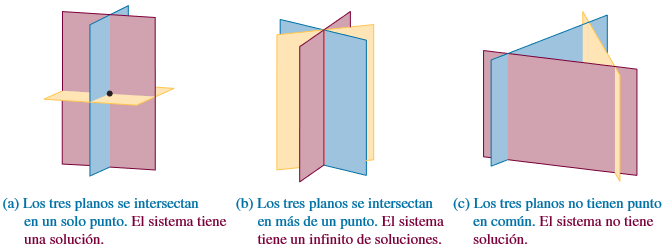
\includegraphics[scale=0.65]{numero-de-soluciones.png}
\caption{Stewart, et. al (2017). \textit{Precálculo. Matemáticas para el Cálculo}. Pp. 643.}
\end{figure}

Profundicemos un poco en la búsqueda de las soluciones de un sistema cuadrado usando matrices.

\subsection{Soluciones de un sistema lineal cuadrado usando matrices.}

En la clase anterior vimos que un sistema de ecuaciones lineales puede ser representado como:
\[
  \vecmat{A} \vecmat{x} = \vecmat{b}
\]
Si el sistema es cuadrado, la matriz $\vecmat{A}$ también lo será y, por tanto, podemos buscar su inversa. Si $\invmat{A}$ existe, significa que el sistema tiene \textbf{una única solución} dada por:
\[
  \vecmat{x} = \invmat{A} \vecmat{b}
\]
En un sistema de $3 \times 3$ quiere decir que los tres planos se intersectan en el punto dado por las componentes de $\invmat{A} \vecmat{b}$.

Ahora, como estudiamos en la clase anterior, la matriz $\invmat{A}$ existe siempre que $\det(\vecmat{A}) \neq 0$. Si el $\det(\vecmat{A}) = 0$ y el sistema es de $3 \times 3$, se abren dos posibilidades para sus soluciones:

\begin{enumerate}
\item Que tenga infinitas soluciones (los planos se cruzan en una misma recta) o
\item Que no tenga solución.
\end{enumerate}

Veamos, como ejemplo, el siguiente \textbf{sistema homogéneo de ecuaciones lineales}\footnote{Un sistema homogéneo es aquel donde los valores de la derecha de las ecuaciones son \textbf{iguales a cero}.}:
\[
\left\{
\begin{aligned}
x + z = 0 \\
x + y = 0 \\
x + 2y + 3z = 0
\end{aligned}
\right.
\]
Este sistema siempre será consistente\footnote{Es decir, tiene al menos una solución.} porque una de sus soluciones es el punto $(0, \ 0, \ 0)$, también conocida como ``solución trivial''.

Es posible que el sistema homogéneo de arriba tenga más de una solución. Aquello se puede evaluar mediante el determinante de su matriz de coeficientes $\vecmat{A}$.

Si el $\det(\vecmat{A}) \neq 0$, entonces existe $\invmat{A}$ y su solución será el vector $\vecmat{0}$.
\[
  \vecmat{x} = \invmat{A} \cdot \vecmat{0} = \vecmat{0}
\]
En otras palabras, los tres planos del sistema se intersectan en el origen.

En cambio, si el $\det(\vecmat{A}) = 0$ quiere decir que este sistema homogéneo tiene \textbf{infinitas soluciones}, las que forman una recta en la intersección de los planos. Otra forma de interpretar este caso, es considerar a las filas de $\vecmat{A}$ como los vectores normales de los tres planos.
\[
  \det(\vecmat{A}) = \det(\vecmat{n}_{1}, \ \vecmat{n}_{2}, \ \vecmat{n}_{3}) = 0
\]
Como el $\det(\vecmat{n}_{1}, \ \vecmat{n}_{2}, \ \vecmat{n}_{3}) = 0$, significa que los tres vectores forman un paralelelpipedo sin volumen o un plano del cual son parte.

Si graficamos a $\vecmat{n}_{1}$, $\vecmat{n}_{2}$ y $\vecmat{n}_{3}$ en sus planos mientras se intersectan, al calcular el producto cruz entre dos de ellos veremos que será un vector paralelo a la recta de las soluciones, lo que significa que es ortogonal a los $\vecmat{n}_{i}$ y paralelo a los planos.

Así, las soluciones de un sistema $\vecmat{A}\vecmat{x} = \vecmat{b}$ de $3 \times 3$ se pueden resumir como:

\begin{table}[hbt!]
\centering

\renewcommand{\arraystretch}{1.3}
\begin{tabular}{c c c c}
\hline
$\det(\vecmat{A})$ & Cantidad de Soluciones & Solución & Intersección de los tres planos \\
\hline
$\neq 0$ & Una & $\vecmat{x} = \invmat{A} \vecmat{b}$ & En un punto \\
$= 0$ & Infinitas & - & En una recta \\
$= 0$ & Ninguna & - & No coinciden en un lugar \\
\hline
\end{tabular}

\end{table}


\end{document}
